% Versión de congreso (Springer LNCS). Compilar desde esta carpeta:  latexmk -pdf paper.tex
% Las cifras vienen de ../numeros.tex y las filas de tablas de ../tablas.tex (generadas por ../analisis.py).
\documentclass[runningheads]{llncs}
\usepackage[T1]{fontenc}
\usepackage[utf8]{inputenc}
\usepackage[spanish,es-tabla,es-nodecimaldot]{babel}
\usepackage{amsmath,amssymb}
\usepackage{graphicx}
\usepackage{booktabs}
\usepackage{xcolor}
\usepackage{tikz}
\usetikzlibrary{arrows.meta,positioning}
\usepackage[hidelinks]{hyperref}
\definecolor{azulm}{HTML}{2E6DB4}\definecolor{naranjam}{HTML}{D9731A}
\definecolor{verdem}{HTML}{2F9467}\definecolor{grism}{HTML}{5A6772}
\graphicspath{{../figuras/}}
% Generado por analisis.py: NO editar a mano.
\newcommand{\nDatasets}{12}
\newcommand{\nParticiones}{5}
\newcommand{\nCasos}{60}
\newcommand{\relRL}{0{,}96}
\newcommand{\cambioRL}{$-$4{,}4\,\%}
\newcommand{\casosRL}{36/60}
\newcommand{\dsRL}{7/12}
\newcommand{\pRL}{$1{,}000$}
\newcommand{\cambioVsEstRL}{$-$2{,}6\,\%}
\newcommand{\dsVsEstRL}{6/12}
\newcommand{\pVsEstRL}{$1{,}000$}
\newcommand{\peorDsRL}{$+$20{,}9\,\%}
\newcommand{\relKNN}{0{,}76}
\newcommand{\cambioKNN}{$-$24{,}3\,\%}
\newcommand{\casosKNN}{56/60}
\newcommand{\dsKNN}{12/12}
\newcommand{\pKNN}{$0{,}004$}
\newcommand{\cambioVsEstKNN}{$-$13{,}6\,\%}
\newcommand{\dsVsEstKNN}{10/12}
\newcommand{\pVsEstKNN}{$0{,}048$}
\newcommand{\peorDsKNN}{$-$0{,}4\,\%}
\newcommand{\relArbol}{1{,}00}
\newcommand{\cambioArbol}{$+$0{,}1\,\%}
\newcommand{\casosArbol}{34/60}
\newcommand{\dsArbol}{7/12}
\newcommand{\pArbol}{$1{,}000$}
\newcommand{\cambioVsEstArbol}{$+$0{,}1\,\%}
\newcommand{\dsVsEstArbol}{7/12}
\newcommand{\pVsEstArbol}{$1{,}000$}
\newcommand{\peorDsArbol}{$+$5{,}0\,\%}
\newcommand{\relRF}{1{,}00}
\newcommand{\cambioRF}{$+$0{,}5\,\%}
\newcommand{\casosRF}{27/60}
\newcommand{\dsRF}{5/12}
\newcommand{\pRF}{$1{,}000$}
\newcommand{\cambioVsEstRF}{$+$0{,}5\,\%}
\newcommand{\dsVsEstRF}{5/12}
\newcommand{\pVsEstRF}{$1{,}000$}
\newcommand{\peorDsRF}{$+$4{,}1\,\%}
\newcommand{\cambioSintRL}{$-$1{,}3\,\%}
\newcommand{\pSintRL}{$0{,}705$}
\newcommand{\dsSintRL}{7/12}
\newcommand{\relSintRL}{0{,}99}
\newcommand{\cambioSintKNN}{$-$0{,}3\,\%}
\newcommand{\pSintKNN}{$0{,}705$}
\newcommand{\dsSintKNN}{7/12}
\newcommand{\relSintKNN}{1{,}00}
\newcommand{\cambioSintArbol}{$+$0{,}3\,\%}
\newcommand{\pSintArbol}{$1{,}000$}
\newcommand{\dsSintArbol}{7/12}
\newcommand{\relSintArbol}{1{,}00}
\newcommand{\cambioSintRF}{$-$0{,}1\,\%}
\newcommand{\pSintRF}{$1{,}000$}
\newcommand{\dsSintRF}{7/12}
\newcommand{\relSintRF}{1{,}00}
\newcommand{\cambioRedRL}{$+$1{,}8\,\%}
\newcommand{\pRedRL}{$0{,}380$}
\newcommand{\dsRedRL}{5/12}
\newcommand{\relRedRL}{1{,}02}
\newcommand{\cambioRedKNN}{$+$1{,}0\,\%}
\newcommand{\pRedKNN}{$0{,}330$}
\newcommand{\dsRedKNN}{4/12}
\newcommand{\relRedKNN}{1{,}01}
\newcommand{\cambioRedArbol}{$+$1{,}4\,\%}
\newcommand{\pRedArbol}{$0{,}330$}
\newcommand{\dsRedArbol}{3/12}
\newcommand{\relRedArbol}{1{,}01}
\newcommand{\cambioRedRF}{$+$2{,}8\,\%}
\newcommand{\pRedRF}{$0{,}049$}
\newcommand{\dsRedRF}{1/12}
\newcommand{\relRedRF}{1{,}03}
\newcommand{\dimMedia}{83\,\%}
\newcommand{\fracEliminados}{22\,\%}
\newcommand{\dimMin}{38\,\%}
\newcommand{\dimMax}{92\,\%}
\newcommand{\mMedia}{0{,}4}
\newcommand{\fracConSintesis}{25\,\%}
\newcommand{\tauMediana}{0{,}18}
\newcommand{\casosNmenosUno}{38/60}
\newcommand{\wLat}{2{,}91}
\newcommand{\wLon}{2{,}85}
\newcommand{\wPop}{0{,}03}
\newcommand{\wInc}{0{,}41}
\newcommand{\fracApagados}{10\,\%}
\newcommand{\nCompCasos}{60}
\newcommand{\compMLKRRL}{$-$1{,}8\,\%}
\newcommand{\compMLKRKNN}{$-$22{,}5\,\%}
\newcommand{\compMLKRArbol}{$+$2{,}0\,\%}
\newcommand{\compMLKRRF}{$+$2{,}6\,\%}
\newcommand{\rangoMLKR}{5{,}7}
\newcommand{\compPGRL}{$-$15{,}7\,\%}
\newcommand{\compPGKNN}{$-$18{,}0\,\%}
\newcommand{\compPGArbol}{$+$0{,}7\,\%}
\newcommand{\compPGRF}{$+$0{,}8\,\%}
\newcommand{\rangoPG}{4{,}6}
\newcommand{\compYJMVRL}{$+$2{,}4\,\%}
\newcommand{\compYJMVKNN}{$-$14{,}5\,\%}
\newcommand{\compYJMVArbol}{$+$1{,}5\,\%}
\newcommand{\compYJMVRF}{$+$1{,}7\,\%}
\newcommand{\rangoYJMV}{5{,}0}
\newcommand{\compCuantRL}{$+$8{,}1\,\%}
\newcommand{\compCuantKNN}{$-$11{,}8\,\%}
\newcommand{\compCuantArbol}{$+$0{,}1\,\%}
\newcommand{\compCuantRF}{$+$0{,}0\,\%}
\newcommand{\rangoCuant}{6{,}4}
\newcommand{\compEstPCARL}{$-$1{,}8\,\%}
\newcommand{\compEstPCAKNN}{$-$12{,}4\,\%}
\newcommand{\compEstPCAArbol}{$-$0{,}6\,\%}
\newcommand{\compEstPCARF}{$-$1{,}9\,\%}
\newcommand{\rangoEstPCA}{4{,}6}
\newcommand{\compPCAnoventaRL}{$+$0{,}6\,\%}
\newcommand{\compPCAnoventaKNN}{$-$10{,}4\,\%}
\newcommand{\compPCAnoventaArbol}{$+$19{,}3\,\%}
\newcommand{\compPCAnoventaRF}{$+$17{,}9\,\%}
\newcommand{\rangoPCAnoventa}{8{,}1}
\newcommand{\compPCAcvRL}{$-$1{,}0\,\%}
\newcommand{\compPCAcvKNN}{$-$12{,}0\,\%}
\newcommand{\compPCAcvArbol}{$+$18{,}7\,\%}
\newcommand{\compPCAcvRF}{$+$15{,}1\,\%}
\newcommand{\rangoPCAcv}{7{,}4}
\newcommand{\compPsrRL}{$-$6{,}1\,\%}
\newcommand{\compPsrKNN}{$-$25{,}0\,\%}
\newcommand{\compPsrArbol}{$-$1{,}1\,\%}
\newcommand{\compPsrRF}{$-$2{,}3\,\%}
\newcommand{\rangoPsr}{3{,}2}
\newcommand{\compPRL}{$-$4{,}4\,\%}
\newcommand{\compPKNN}{$-$24{,}3\,\%}
\newcommand{\compPArbol}{$+$0{,}1\,\%}
\newcommand{\compPRF}{$+$0{,}5\,\%}
\newcommand{\rangoP}{4{,}7}
\newcommand{\mejorAlt}{estándar + PCA}
\newcommand{\rangoMejorAlt}{4{,}6}
\newcommand{\nReps}{10}
\newcommand{\vMedia}{0{,}80}
\newcommand{\vFracUno}{22\,\%}
\newcommand{\nSintMedia}{3{,}9}
\newcommand{\ctrlIniAleat}{$+$0{,}6\,\%}
\newcommand{\pCtrlIniAleat}{$1{,}000$}
\newcommand{\ctrlIniAleatRL}{$+$1{,}7\,\%}
\newcommand{\ctrlSigmaBajo}{$+$0{,}5\,\%}
\newcommand{\pCtrlSigmaBajo}{$1{,}000$}
\newcommand{\ctrlSigmaBajoRL}{$-$0{,}1\,\%}
\newcommand{\ctrlSigmaAlto}{$+$0{,}9\,\%}
\newcommand{\pCtrlSigmaAlto}{$1{,}000$}
\newcommand{\ctrlSigmaAltoRL}{$-$0{,}4\,\%}
\newcommand{\ctrlPobDoble}{$+$0{,}2\,\%}
\newcommand{\pCtrlPobDoble}{$1{,}000$}
\newcommand{\ctrlPobDobleRL}{$-$0{,}2\,\%}
\newcommand{\nAblCasos}{24}
\newcommand{\ctrlPesos}{$+$2{,}2\,\%}
\newcommand{\ctrlPesosRL}{$+$6{,}5\,\%}
\newcommand{\pCtrlPesos}{$0{,}424$}
\newcommand{\ctrlExp}{$+$10{,}0\,\%}
\newcommand{\ctrlExpRL}{$+$2{,}2\,\%}
\newcommand{\pCtrlExp}{$0{,}012$}
\newcommand{\ctrlAleat}{$+$6{,}2\,\%}
\newcommand{\ctrlAleatRL}{$+$3{,}0\,\%}
\newcommand{\pCtrlAleat}{$0{,}012$}
\newcommand{\ctrlMI}{$+$14{,}9\,\%}
\newcommand{\ctrlMIRL}{$+$6{,}8\,\%}
\newcommand{\pCtrlMI}{$0{,}012$}
\newcommand{\ctrlYJMI}{$+$11{,}0\,\%}
\newcommand{\ctrlYJMIRL}{$+$10{,}3\,\%}
\newcommand{\pCtrlYJMI}{$0{,}014$}
\newcommand{\nCtrlCasos}{24}
\newcommand{\rangoCeroR}{$+$2{,}2\,\%}
\newcommand{\pRangoCero}{$1{,}000$}
\newcommand{\dsPeorRangoCero}{7}
\newcommand{\rangoUnoR}{$+$0{,}3\,\%}
\newcommand{\pRangoUno}{$1{,}000$}
\newcommand{\dsPeorRangoUno}{6}
\newcommand{\rangoCuatroR}{$+$0{,}5\,\%}
\newcommand{\pRangoCuatro}{$1{,}000$}
\newcommand{\dsPeorRangoCuatro}{7}
\newcommand{\rangoOchoR}{$+$1{,}7\,\%}
\newcommand{\pRangoOcho}{$0{,}256$}
\newcommand{\dsPeorRangoOcho}{9}
\newcommand{\bordeUno}{11\,\%}
\newcommand{\bordeDos}{7\,\%}
\newcommand{\bordeCuatro}{8\,\%}
\newcommand{\bordeOcho}{5\,\%}
\newcommand{\nRango}{24}
\newcommand{\mleFueraDos}{24\,\%}
\newcommand{\nAlgCasos}{24}
\newcommand{\rangoCMA}{1{,}9}
\newcommand{\algMejor}{CMA-ES}
\newcommand{\algKNNcma}{$-$25{,}7\,\%}
\newcommand{\algKNNaleat}{$-$21{,}0\,\%}
\newcommand{\algKNNmin}{$-$24{,}8\,\%}
\newcommand{\algKNNmax}{$-$23{,}3\,\%}
\newcommand{\segMediana}{191}
\newcommand{\segMax}{243}
\newcommand{\msPorEval}{191}
\newcommand{\segMLKR}{16{,}8}
\newcommand{\segPG}{6{,}1}
\newcommand{\segYJMV}{0{,}6}
\newcommand{\popMin}{11}
\newcommand{\popMax}{13}
\newcommand{\muMin}{5}
\newcommand{\muMax}{6}
\newcommand{\muEffMin}{3{,}4}
\newcommand{\muEffMax}{4{,}0}
\newcommand{\genMin}{77}
\newcommand{\genMax}{91}
\newcommand{\nParadaPresupuesto}{12}
\newcommand{\nParadaTotal}{12}
\newcommand{\evalMejorMediana}{971}
\newcommand{\evalMejorMin}{658}
\newcommand{\mejoraFitnessMediana}{$-$12{,}1\,\%}
\newcommand{\sigmaFinMin}{0{,}007}
\newcommand{\sigmaFinMax}{0{,}06}
\newcommand{\cribSelRL}{$-$2{,}5\,\%}
\newcommand{\cribSelKNN}{$-$23{,}9\,\%}
\newcommand{\cribSelArbol}{$+$0{,}1\,\%}
\newcommand{\cribSelRF}{$+$0{,}8\,\%}
\newcommand{\cribDimSel}{72\,\%}
\newcommand{\cribFijoRL}{$-$5{,}4\,\%}
\newcommand{\cribFijoKNN}{$-$25{,}0\,\%}
\newcommand{\cribFijoArbol}{$-$0{,}5\,\%}
\newcommand{\cribFijoRF}{$+$0{,}0\,\%}
\newcommand{\cribDimFijo}{89\,\%}
\newcommand{\cribPcaRL}{$-$2{,}7\,\%}
\newcommand{\cribPcaKNN}{$-$23{,}9\,\%}
\newcommand{\cribPcaArbol}{$+$0{,}8\,\%}
\newcommand{\cribPcaRF}{$+$1{,}9\,\%}
\newcommand{\cribDimPca}{70\,\%}
\newcommand{\cribFijoNoReduce}{27/60}
% Generado por analisis.py: filas de las tablas (una macro por tabla).
\newcommand{\filasPrincipal}{%
R. lineal & 0{,}98 & 0{,}94 & \textbf{0{,}96} & 7/12 & $1{,}000$ & $-$2{,}6\,\%\\
KNN & 0{,}88 & 0{,}75 & \textbf{0{,}76} & 12/12 & $0{,}004$ & $-$13{,}6\,\%\\
Árbol & 1{,}00 & 0{,}99 & \textbf{1{,}00} & 7/12 & $1{,}000$ & $+$0{,}1\,\%\\
RF & 1{,}00 & 0{,}98 & \textbf{1{,}00} & 5/12 & $1{,}000$ & $+$0{,}5\,\%\\
}
\newcommand{\filasDimension}{%
diabetes & 10 & 8{,}0 & 0{,}6 & 8{,}6 & 0{,}46\\
concrete & 8 & 6{,}6 & 0{,}0 & 6{,}6 & 0{,}47\\
stock & 9 & 7{,}6 & 0{,}4 & 8{,}0 & 0{,}30\\
space\_ga & 6 & 3{,}8 & 0{,}4 & 4{,}2 & 0{,}09\\
sulfur & 6 & 5{,}0 & 0{,}0 & 5{,}0 & 0{,}01\\
wine\_quality & 11 & 9{,}6 & 0{,}2 & 9{,}8 & 0{,}41\\
kin8nm & 8 & 7{,}0 & 0{,}0 & 7{,}0 & 0{,}34\\
bank8FM & 8 & 6{,}8 & 0{,}2 & 7{,}0 & 0{,}05\\
puma8NH & 8 & 2{,}2 & 2{,}4 & 4{,}6 & 1{,}83\\
house\_8L & 8 & 7{,}0 & 0{,}0 & 7{,}0 & 0{,}12\\
cpu\_small & 12 & 10{,}8 & 0{,}2 & 11{,}0 & 0{,}19\\
california & 8 & 6{,}6 & 0{,}0 & 6{,}6 & 0{,}02\\
}
\newcommand{\filasComparativa}{%
estándar & 0{,}98 & 0{,}88$^*$ & 1{,}00 & 1{,}00 & 5{,}3 & 1{,}00\\
YJ máx.\ verosimilitud & 1{,}02 & 0{,}85$^*$ & 1{,}01 & 1{,}02 & 5{,}0 & 1{,}00\\
cuantiles & 1{,}08 & 0{,}88$^*$ & 1{,}00 & 1{,}00 & 6{,}4 & 1{,}00\\
solo PCA (95\,\%) & 1{,}01 & 0{,}90$^*$ & 1{,}19$^*$ & 1{,}18$^*$ & 8{,}1 & 0{,}79\\
solo PCA (\% por VC) & 0{,}99 & 0{,}88$^*$ & 1{,}19$^*$ & 1{,}15 & 7{,}4 & 0{,}91\\
estándar + su PCA & 0{,}98 & 0{,}88$^*$ & 0{,}99 & 0{,}98 & 4{,}6 & 2{,}00\\
MLKR & 0{,}98 & 0{,}78 & 1{,}02 & 1{,}03 & 5{,}7 & 1{,}00\\
PG (gplearn) & \textbf{0{,}84} & 0{,}82$^*$ & 1{,}01 & 1{,}01 & 4{,}6 & 2{,}00\\
$P$ sin reducir & 0{,}94 & \textbf{0{,}75} & \textbf{0{,}99} & \textbf{0{,}98} & 3{,}2 & 2{,}00\\
\textbf{$P$} & 0{,}96 & 0{,}76 & 1{,}00 & 1{,}00 & 4{,}7 & 0{,}83\\
}
\newcommand{\filasAblacion}{%
\multicolumn{4}{@{}l}{\emph{Piezas}}\\
\quad solo pesos ($\lambda=1$) & $+$2{,}2\,\% & $+$6{,}5\,\% & $-$0{,}1\,\%\\
\quad solo exponentes ($w=1$) & $+$10{,}0\,\%$^*$ & $+$2{,}2\,\% & $+$0{,}4\,\%\\
\midrule
\multicolumn{4}{@{}l}{\emph{Sin búsqueda}}\\
\quad pesos por inf.\ mutua & $+$14{,}9\,\%$^*$ & $+$6{,}8\,\% & $+$3{,}6\,\%\\
\quad YJ (MV) + pesos inf.\ mutua & $+$11{,}0\,\% & $+$10{,}3\,\% & $+$3{,}6\,\%\\
\midrule
\multicolumn{4}{@{}l}{\emph{Búsqueda}}\\
\quad búsqueda aleatoria (1000 puntos) & $+$6{,}2\,\%$^*$ & $+$3{,}0\,\% & $+$2{,}0\,\%\\
\midrule
\multicolumn{4}{@{}l}{\emph{Inicio}}\\
\quad media inicial aleatoria & $+$0{,}6\,\% & $+$1{,}7\,\% & $+$0{,}6\,\%\\
\quad $\sigma_0=0{,}1$ & $+$0{,}5\,\% & $-$0{,}1\,\% & $+$0{,}8\,\%\\
\quad $\sigma_0=0{,}4$ & $+$0{,}9\,\% & $-$0{,}4\,\% & $+$0{,}6\,\%\\
\quad población $\times2$ & $+$0{,}2\,\% & $-$0{,}2\,\% & $+$1{,}3\,\%\\
\midrule
\multicolumn{4}{@{}l}{\emph{Rango}}\\
\quad $\lambda\in[-1,1]$ & $+$0{,}3\,\% & $+$1{,}5\,\% & $-$0{,}3\,\%\\
\quad $\lambda\in[-4,4]$ & $+$0{,}5\,\% & $+$1{,}4\,\% & $+$1{,}1\,\%\\
\quad $\lambda\in[-8,8]$ & $+$1{,}7\,\% & $+$5{,}0\,\% & $+$1{,}4\,\%\\
}
\newcommand{\filasControles}{%
solo pesos ($\lambda=1$) & $+$2{,}2\,\% & $+$6{,}5\,\% & $-$0{,}1\,\%\\
solo exponentes ($w=1$) & $+$10{,}0\,\%$^*$ & $+$2{,}2\,\% & $+$0{,}4\,\%\\
búsqueda aleatoria & $+$6{,}2\,\%$^*$ & $+$3{,}0\,\% & $+$2{,}0\,\%$^*$\\
pesos por inf.\ mutua & $+$14{,}9\,\%$^*$ & $+$6{,}8\,\% & $+$3{,}6\,\%\\
YJ (MV) + pesos inf.\ mutua & $+$11{,}0\,\%$^*$ & $+$10{,}3\,\% & $+$3{,}6\,\%\\
}
\newcommand{\filasAlgoritmos}{%
\textbf{CMA-ES} & 1{,}9 & $-$25{,}7\,\% & $-$7{,}7\,\%\\
AG (propio) & 2{,}8 & $-$24{,}4\,\% & $-$8{,}5\,\%\\
HS & 3{,}2 & $-$24{,}5\,\% & $-$8{,}3\,\%\\
BBO & 4{,}4 & $-$24{,}8\,\% & $-$8{,}0\,\%\\
PSO & 4{,}5 & $-$24{,}1\,\% & $-$5{,}1\,\%\\
DE & 5{,}4 & $-$23{,}3\,\% & $-$5{,}9\,\%\\
ABC & 5{,}9 & $-$24{,}0\,\% & $-$2{,}4\,\%\\
búsqueda aleatoria & 7{,}9 & $-$21{,}0\,\% & $-$4{,}9\,\%\\
}
\newcommand{\filasCoste}{%
P (CMA-ES, 1000 evaluaciones) & 190{,}6 & 242{,}6\\
MLKR & 16{,}8 & 41{,}8\\
PG (gplearn) & 6{,}1 & 14{,}1\\
PCA v-CV & 1{,}0 & 11{,}5\\
YJ máx. verosimilitud & 0{,}6 & 4{,}3\\
cuantiles & 0{,}1 & 0{,}8\\
estándar + PCA & 0{,}0 & 0{,}0\\
}
\newcommand{\filasDatasets}{%
diabetes & 442 & 10\\
concrete & 1\,030 & 8\\
stock & 950 & 9\\
space\_ga & 3\,107 & 6\\
sulfur & 10\,000 & 6\\
wine\_quality & 6\,497 & 11\\
kin8nm & 8\,192 & 8\\
bank8FM & 8\,192 & 8\\
puma8NH & 8\,192 & 8\\
house\_8L & 10\,000 & 8\\
cpu\_small & 8\,192 & 12\\
california & 20\,640 & 8\\
}

\setlength{\textfloatsep}{10pt plus 2pt}

\begin{document}
\title{Forma, relevancia, reducción y síntesis: aprendizaje evolutivo de una representación de atributos más
pequeña para regresión}
\titlerunning{Aprendizaje evolutivo de una representación de atributos más pequeña}
\author{Andrea López Salazar}
\authorrunning{A. López Salazar}
\institute{Universidad Carlos III de Madrid, Máster en Ciencia y Tecnología}
\maketitle

\begin{abstract}
Proponemos un método que aprende, solo con el conjunto de entrenamiento, una transformación de los atributos con
\emph{menos} dimensiones que la original y que reduce el error de modelos de regresión. La transformación tiene
cuatro bloques: un exponente de Yeo-Johnson por atributo (\emph{forma}), un peso por atributo (\emph{relevancia}),
la eliminación de los atributos cuyo peso queda bajo un umbral (\emph{reducción}) y la adición de componentes
principales del espacio aprendido hasta $n-1$ atributos (\emph{síntesis}). CMA-ES optimiza los $2n+2$ parámetros,
umbral incluido, sobre el error de validación cruzada de KNN; la restricción de dimensión se impone en la
decodificación, así que todo individuo es válido. En \nDatasets{} datasets y \nParticiones{} particiones no usadas
en el diseño, la representación usa de media el \dimMedia{} de los atributos y el error baja un \cambioKNN{} en KNN
($p=$\pKNN) y un \cambioRL{} en regresión lineal (no significativo), mientras que en árboles queda igual. Mostramos
que reducir la dimensión y sintetizar direcciones oblicuas compiten: a los árboles les ayuda añadir dimensiones.
\keywords{CMA-ES \and reducción de dimensionalidad \and selección de atributos \and Yeo-Johnson \and KNN}
\end{abstract}

\section{Introducción}
Dado $(X_t,y_t)$, buscamos un programa $P$ que aprenda una transformación $X\mapsto X'=P(X)$ con
$\dim X'<\dim X$ tal que un modelo \emph{arbitrario} $M$ entrenado con $X'_t$ tenga menor error absoluto medio en
validación que entrenado con $X_t$ ($e'<e$), y en la que el criterio para eliminar atributos lo decida el algoritmo
evolutivo. La dificultad está en ``arbitrario'': KNN depende de la geometría (escalas, atributos irrelevantes, colas
largas); la regresión lineal (RL), de la forma de la relación con $y$; un árbol es invariante a cualquier
transformación monótona por atributo y solo cambia si se le dan \emph{direcciones nuevas}.

Contribuciones: (i) una transformación con $2n+2$ parámetros interpretables, optimizada con CMA-ES~\cite{hansen2001},
en la que el umbral de eliminación forma parte del genoma y la restricción $\dim X'<n$ se cumple por construcción;
(ii) una evaluación en dos fases (exploración y confirmación con particiones nuevas) en 12 datasets y cuatro familias
de modelos, con estadística por dataset; (iii) un análisis de la tensión entre reducir y sintetizar.

\section{Trabajos relacionados}
Ponderar atributos para KNN es una idea clásica~\cite{wettschereck1997}, y los algoritmos genéticos se han usado
para aprender esos pesos y seleccionar atributos~\cite{raymer2000}. El aprendizaje de métricas generaliza la
ponderación a una matriz de Mahalanobis completa~\cite{weinberger2009}, con $O(n^2)$ parámetros y sin corregir la
forma de cada atributo. Las transformaciones de potencia (Yeo-Johnson~\cite{yeo2000}) se ajustan normalmente por
máxima verosimilitud, buscando normalidad; aquí sus exponentes se eligen para predecir. Añadir componentes
principales para dar cortes oblicuos a los árboles es la idea de Rotation Forest~\cite{rodriguez2006}. Para la
búsqueda comparamos CMA-ES con metaheurísticas bioinspiradas~\cite{fister2013}.

\section{Método}
\subsection{Transformación}
Para cada atributo $j$, con $\psi(\cdot;\lambda)$ la transformación de Yeo-Johnson y $\mu_j,\sigma_j$ calculadas
\emph{solo} en el entrenamiento:
\begin{equation}
z_j = w_j\,\frac{\psi(x_j;\lambda_j)-\mu_j}{\sigma_j},\qquad S=\{j: w_j\ge\tau\},\qquad
X'=\big[\,z_S\;\big|\;V_m^\top(z_S-\bar z_S)\,\big],
\end{equation}
con $\lambda_j\in[-2,2]$, $w_j,\tau\in[0,3]$, $V_m$ las $m$ primeras componentes principales de $z_S$ en el
entrenamiento y $m=\mathrm{round}(\rho\,(n-1-|S|))$, $\rho\in[0,1]$. Si $|S|=n$ se elimina además el atributo de
menor peso, y si $|S|=0$ se conserva el de mayor peso. Así $\dim X'=|S|+m\le n-1$ para \emph{cualquier} $\theta$
(Fig.~\ref{fig:esquema}). El punto de partida $\theta_0$ es la estandarización ($\lambda=w=\mathbf 1$) con
$\tau_0=\rho_0=0{,}5$.

\begin{figure}[t]\centering\def\esquemaescala{0.8}
% Esquema del método P, compartido por memoria, paper y póster.
% Requiere: tikz con las librerías arrows.meta y positioning; colores azulm, naranjam, verdem, grism.
% \esquemaescala permite reducirlo o ampliarlo sin tocar el dibujo.
\providecommand{\esquemaescala}{1}
\begin{tikzpicture}[scale=\esquemaescala, every node/.style={transform shape},
  node distance=3.5mm and 3.5mm,
  caja/.style={draw=azulm, rounded corners=2pt, fill=azulm!8, align=center, inner sep=2.5pt,
               minimum height=9mm, font=\footnotesize},
  sint/.style={caja, draw=verdem, fill=verdem!10},
  red/.style={caja, draw=naranjam, fill=naranjam!8},
  fl/.style={-{Stealth[length=2mm]}, thick, azulm!80!black},
  fv/.style={fl, verdem!80!black},
  fn/.style={fl, naranjam!80!black}]
% fila 1: bloques por atributo (forma, escala, relevancia)
\node (x) {$x_j$};
\node[caja, right=of x]   (yj) {1. Forma\\$\psi(x_j;\lambda_j)$};
\node[caja, right=of yj]  (st) {Escala\\$(\psi_j-\mu_j)/\sigma_j$};
\node[caja, right=of st]  (w)  {2. Relevancia\\$\times\,w_j$};
\node[right=of w] (z) {$z_j$};
\draw[fl] (x)--(yj); \draw[fl] (yj)--(st); \draw[fl] (st)--(w); \draw[fl] (w)--(z);
% fila 2: reducción, síntesis y salida
\node[red, below=7mm of st] (sel) {3. Reducción\\$S=\{j: w_j\ge\tau\}$};
\node[sint, right=5mm of sel] (pca) {4. Síntesis\\$p_{1..m}=V_m^{\top}(z_S-\bar z_S)$};
\node[draw=grism, thick, rounded corners=2pt, fill=white, font=\footnotesize, minimum height=7mm, align=center,
     below=5mm of pca] (xp) {$X'=[\,z_S\;|\;p_1\ldots p_m\,]$,\; $|S|+m\le n-1$};
\draw[fn] (z.south) |- ([yshift=3.5mm]sel.north) -- (sel.north);
\draw[fv] (sel.east) -- (pca.west);
\draw[fv] (pca.south) -- (xp.north);
\draw[fn] (sel.south) |- (xp.west);
\node[font=\scriptsize\itshape, text=grism, align=right, anchor=east] at ([xshift=-3mm]sel.west)
     {si $|S|=n$, fuera\\el de menor $w_j$};
\node[font=\scriptsize\itshape, text=grism, align=left, anchor=west] at ([xshift=2mm]pca.east)
     {$m=\mathrm{round}(\rho\,(n{-}1{-}|S|))$};
% búsqueda
\node[caja, draw=naranjam, fill=naranjam!10, above=6mm of st, align=center] (cma)
     {CMA-ES busca $\theta=(\lambda,w,\tau,\rho)$:\; $\lambda_j\in[-2,2]$,\; $w_j,\tau\in[0,3]$,\; $\rho\in[0,1]$\\
      minimizando el MAE de validación cruzada de KNN en el entrenamiento};
\draw[fn] (cma.south -| yj) -- (yj.north);
\draw[fn] (cma.south -| w) -- (w.north);
\end{tikzpicture}

\caption{El programa $P$. CMA-ES ajusta forma, relevancia, el umbral de eliminación $\tau$ y la fracción de síntesis
$\rho$; la decodificación garantiza $\dim X'\le n-1$.}
\label{fig:esquema}
\end{figure}

\begin{proposition}
Sea $\tilde z=[z,V^\top(z-\bar z)]$ con $V$ ortogonal y \emph{todas} las componentes. Entonces (a)
$\lVert\tilde z-\tilde z'\rVert^2=2\lVert z-z'\rVert^2$, por lo que KNN obtiene los mismos vecinos; (b) el espacio
columna de $[\mathbf 1, Z, (Z-\bar z)V]$ coincide con el de $[\mathbf 1,Z]$, por lo que la RL da las mismas
predicciones.
\end{proposition}
\begin{proof}
(a) $\lVert V^\top(z-z')\rVert=\lVert z-z'\rVert$ por ortogonalidad. (b) $(Z-\bar z)V=ZV-\mathbf 1\bar z^\top V$ es
combinación lineal de las columnas de $Z$ y de $\mathbf 1$.\qed
\end{proof}
La síntesis completa, por tanto, solo cambia a los árboles, pero duplica la dimensión ($P$ sin reducir, que usamos
como referencia). Con $\dim X'<n$ la síntesis compite por el hueco con los atributos originales y la decide el
fitness.

\subsection{Fitness y búsqueda}
El fitness de $\theta=(\lambda,w,\tau,\rho)$ es el MAE de validación cruzada (5 pliegues fijos) de KNN ($k=5$) en
$X'$, dividido por el MAE del predictor constante (la mediana), sobre una submuestra de hasta 2000 filas del
entrenamiento. No es derivable (depende de qué puntos son vecinos y tiene escalones en $\tau$) y es ruidoso, lo que
motiva CMA-ES: selección por rango (invariante a transformaciones monótonas del fitness), recombinación intermedia
de los $\mu$ mejores (promedia el ruido) y adaptación de la covarianza (aprende qué genes se mueven juntos: el peso y
el exponente de un atributo, el umbral y los pesos). Optimizamos en $[0,1]^{2n+2}$ reescalado a los límites, con
$\sigma_0=0{,}2$, población por defecto $4+\lfloor3\ln D\rfloor$ y 1000 evaluaciones. No hay penalización por
dimensión: CMA-ES decide qué atributos sobran (los de menor peso) y cuántos (el umbral), y eliminar más de los
necesarios solo compensa si mejora el fitness.

\section{Diseño experimental}
Usamos 12 datasets de regresión: los dos de la práctica (diabetes y california) y diez de OpenML (concrete, stock,
space\_ga, sulfur, kin8nm, bank8FM, puma8NH, house\_8L, cpu\_small, wine\_quality) con 6--12 atributos numéricos y
como mucho 10\,000 filas. Las variantes del método se exploraron con otras semillas; el experimento de confirmación
usa 5 particiones 70/30 nuevas (semillas 40--44), \nCasos{} casos por modelo. Modelos fijos y sin ajustar: RL, KNN
($k=5$), árbol de decisión y Random Forest (RF, 100 árboles). Como las particiones de un dataset comparten filas, la
unidad estadística es el dataset ($n=12$): $e'/e$ se resume con medias geométricas y se contrasta con Wilcoxon y
corrección de Holm; las comparaciones múltiples, con Friedman y Nemenyi~\cite{demsar2006}.

\section{Resultados}
\subsection{Resultado principal}
\begin{table}[tb]\centering\setlength{\tabcolsep}{5pt}
\caption{$e'/e$ (media geométrica de los 12 datasets). \emph{Datasets}: con $e'<e$; $p$: Wilcoxon por dataset con
Holm; última columna: cambio de $P$ frente a $X$ estandarizado.}
\label{tab:principal}
\begin{tabular}{@{}lcccccc@{}}\toprule
Modelo & estándar & $P$ sin reducir ($2n$) & $P$ ($<n$) & Datasets & $p$ & vs.\ est.\\\midrule
\filasPrincipal\bottomrule
\end{tabular}
\end{table}

$X'$ usa de media el \dimMedia{} de los atributos y siempre menos de $n$. Con esa representación más pequeña
(Tabla~\ref{tab:principal}, Fig.~\ref{fig:principal}), KNN mejora \cambioKNN{} frente a $X$ original ($p=$\pKNN,
\dsKNN{} datasets) y \cambioVsEstKNN{} frente a estandarizar ($p=$\pVsEstKNN). La RL mejora \cambioRL{} sin
significación, y los árboles quedan igual (árbol \cambioArbol, RF \cambioRF).

\begin{figure}[tb]\centering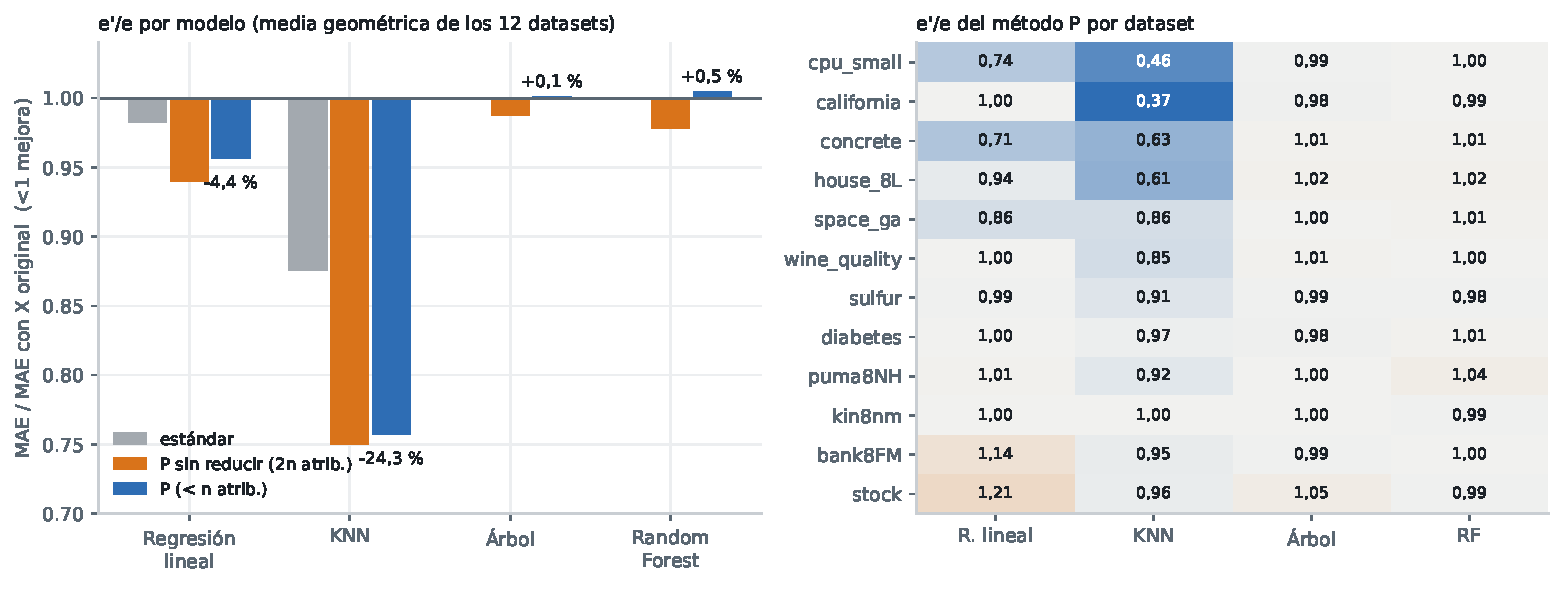
\includegraphics[width=\textwidth]{principal}
\caption{Izquierda: $e'/e$ por modelo. Derecha: $e'/e$ de $P$ por dataset (azul: mejora; naranja: empeora).}
\label{fig:principal}
\end{figure}

\subsection{Reducción de dimensionalidad}
\begin{table}[tb]\centering\setlength{\tabcolsep}{6pt}
\caption{Reducción aprendida (media de 5 particiones): $n$ atributos, $s$ conservados, $m$ componentes
sintetizadas, $\dim X'$ y umbral $\tau$ (mediana).}
\label{tab:dimension}\scriptsize
\begin{tabular}{@{}lccccc@{}}\toprule
Dataset & $n$ & $s$ & $m$ & $\dim X'$ & $\tau$\\\midrule
\filasDimension\bottomrule
\end{tabular}
\end{table}
CMA-ES elimina el \fracEliminados{} de los atributos originales (Tabla~\ref{tab:dimension}), con un umbral mediano
$\tau=$\tauMediana; en puma8NH conserva 2 y añade componentes. Frente a $P$ sin reducir ($2n$), reducir cambia el
error de KNN \cambioRedKNN{} y el de RL \cambioRedRL{} (no significativos), pero empeora RF un \cambioRedRF{}
($p=$\pRedRF): pierde las direcciones oblicuas. Dentro del presupuesto de $n-1$, CMA-ES solo sintetiza en el
\fracConSintesis{} de las particiones y quitar la síntesis apenas cambia nada (RF \cambioSintRF): con un fitness de
KNN el hueco no se dedica a los árboles. Fijar el umbral fuera de la evolución da resultados parecidos con una regla
de un error estándar (KNN \cribSelKNN), pero un umbral fijo $w_j<0{,}1$ no reduce en \cribFijoNoReduce{} particiones.

\subsection{Comparativa}
\begin{table}[tb]\centering\setlength{\tabcolsep}{4pt}
\caption{Comparativa en las mismas particiones: $e'/e$ (negrita: mejor; $^*$: $P$ mejor con $p<0{,}05$, Wilcoxon por
dataset con Holm), rango medio de Friedman (1 = mejor) y dimensión relativa $d/n$.}
\label{tab:comparativa}\scriptsize
\begin{tabular}{@{}lcccccc@{}}\toprule
Transformación & R.\ lin. & KNN & Árbol & RF & Rango & $d/n$\\\midrule
\filasComparativa\bottomrule
\end{tabular}
\end{table}
Comparamos con estandarizar, Yeo-Johnson por máxima verosimilitud, cuantiles, ``solo PCA'' (95\,\% de varianza o \%
elegido por validación cruzada), añadir la PCA de $X$ estandarizado, MLKR y programación genética (\texttt{gplearn}).
Las tres transformaciones con mejor rango medio usan $2n$ atributos; \textbf{entre las que no aumentan la dimensión,
$P$ es la mejor} (rango \rangoP) y la única que reduce sin dañar a los árboles: ``solo PCA'' empeora a RF un
\compPCAnoventaRF{} (Tabla~\ref{tab:comparativa}, Fig.~\ref{fig:sintesis}).

\begin{figure}[tb]\centering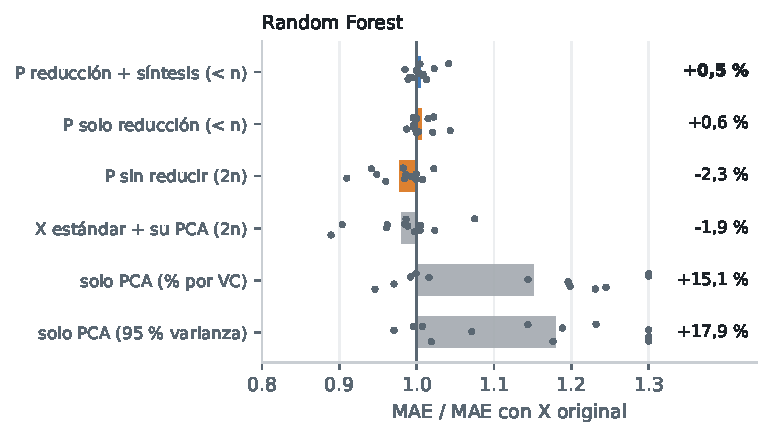
\includegraphics[width=0.7\textwidth]{sintesis_rf}
\caption{Random Forest en las mismas particiones: a los árboles les ayuda \emph{añadir} direcciones oblicuas ($2n$);
sustituir los ejes por componentes los empeora.}
\label{fig:sintesis}
\end{figure}

\subsection{La búsqueda}
Cambiando una decisión de la búsqueda de $(\lambda,w)$ cada vez (\nAblCasos{} particiones), los pesos son la pieza principal (quitar
los exponentes cuesta poco; fijar $w=1$, un \ctrlExp{} en KNN) y la búsqueda gana a la aleatoria (\ctrlAleat) y a
los pesos por información mutua (\ctrlMI). CMA-ES es robusto a la población inicial y al rango de los exponentes.
Con el mismo $\theta$, fitness y presupuesto, CMA-ES obtiene el mejor rango de fitness (\rangoCMA) entre siete
optimizadores, pero las metaheurísticas quedan cerca y solo la búsqueda aleatoria es claramente peor.

\subsection{Coste y caso negativo}
Una búsqueda tarda \segMediana\,s de mediana por partición y se paga una vez por dataset. En diabetes (309 filas de
entrenamiento) el fitness mejora pero la validación no de forma fiable: sobreajuste al criterio de búsqueda.

\section{Conclusiones}
Una transformación con forma, relevancia, reducción y síntesis, aprendida con CMA-ES solo sobre el entrenamiento,
cumple $\dim X'<n$ con un umbral de eliminación aprendido y reduce el error de KNN de forma concluyente y el de RL en
media. La restricción de dimensión revela una tensión: lo que ayuda a los árboles es añadir direcciones, no
quitarlas. Limitaciones: datos numéricos de tamaño medio, sobreajuste con pocos datos y un fitness que solo mira a
KNN. Queda optimizar para varias familias a la vez, para que el presupuesto de atributos se reparta entre originales
y componentes.

\begin{thebibliography}{10}
\bibitem{hansen2001} Hansen, N., Ostermeier, A.: Completely derandomized self-adaptation in evolution strategies.
Evolutionary Computation \textbf{9}(2), 159--195 (2001)
\bibitem{yeo2000} Yeo, I.K., Johnson, R.A.: A new family of power transformations to improve normality or symmetry.
Biometrika \textbf{87}(4), 954--959 (2000)
\bibitem{wettschereck1997} Wettschereck, D., Aha, D.W., Mohri, T.: A review and empirical evaluation of feature
weighting methods for a class of lazy learning algorithms. Artif. Intell. Rev. \textbf{11}, 273--314 (1997)
\bibitem{raymer2000} Raymer, M.L., Punch, W.F., Goodman, E.D., Kuhn, L.A., Jain, A.K.: Dimensionality reduction using
genetic algorithms. IEEE Trans. Evol. Comput. \textbf{4}(2), 164--171 (2000)
\bibitem{weinberger2009} Weinberger, K.Q., Saul, L.K.: Distance metric learning for large margin nearest neighbor
classification. J. Mach. Learn. Res. \textbf{10}, 207--244 (2009)
\bibitem{rodriguez2006} Rodríguez, J.J., Kuncheva, L.I., Alonso, C.J.: Rotation forest: a new classifier ensemble
method. IEEE Trans. Pattern Anal. Mach. Intell. \textbf{28}(10), 1619--1630 (2006)
\bibitem{fister2013} Fister Jr., I., Yang, X.S., Fister, I., Brest, J., Fister, D.: A brief review of
nature-inspired algorithms for optimization. Elektrotehniški vestnik \textbf{80}(3), 1--7 (2013)
\bibitem{demsar2006} Demšar, J.: Statistical comparisons of classifiers over multiple data sets. J. Mach. Learn.
Res. \textbf{7}, 1--30 (2006)
\end{thebibliography}
\end{document}
